%% Richard Wen
%% rwen@ryerson.ca


% *** INTRODUCTION ***


\section{Introduction} \label{introduction}

The wide availability of mobile devices have enabled millions of people to share online content, such as text, images, sound, and videos, from any location with wireless Internet connection. Social media platforms, such as Facebook \citep{Facebook:2017} and Twitter \citep{Twitter:2017}, are commonly used to share large amounts of online content in near real-time. This online content produces valuable sources of real-time locational data, known as geosocial media data, that may provide information on current real-world events such as traffic jams, natural disasters, disease spread, and terrorist attacks. Geosocial media data can be used to detect and predict real-world events given particular locations and times. However, human errors, inconsistencies, noise, high volumes, and constant changes make it difficult to extract useful information from geosocial media data. These issues cause a divide in the methods and approaches for geosocial media event detection and prediction, where standards, comparisons, and integration between different data sources and use cases are rare. This proposal documents a plan to develop a generalized framework and open source software for detecting and predicting real-world events using geosocial media data.

The objective of this proposal is to develop a framework and accompanying software to detect and predict real-world events in real-time with geosocial media data. A literature review was done to provide background knowledge on current research on event detection and prediction methods and applications. An approach, built on the knowledge from the literature review, was developed to satisfy the objectives. Recent progress was detailed to provide preliminary results and relevant past work related to the objectives. A discussion of the impacts was provided to address the importance and effect of the proposed research work.

The remaining sections are organized as follows:

\begin{itemize}
	\item \textbf{Section \ref{objectives}} details the objectives of the proposed research
	\item \textbf{Section \ref{literature-review}} provides a literature review of current research
	\item \textbf{Section \ref{approach}} details the proposed approach to satisfy the objectives
	\item \textbf{Section \ref{recent-progress}} details the recent progress based on the approaches and objectives
	\item \textbf{Section \ref{impact}} discusses the impact of the proposed research
	\item \textbf{Section \ref{conclusion}} provides concluding summaries and remarks
\end{itemize}

\section{Objectives} \label{objectives}

This section provides details objectives of this proposal. The main objective is to develop the following for detecting and predicting real-world events using geosocial media data:

\begin{enumerate}
	\item Framework that can be applied to a wide variety of applications and data
	\item Open Source Software based on (1)
\end{enumerate}

\subsection{Framework} \label{framework}

The framework objective requires that the following components be identified and developed:

\begin{itemize}
	\item \textbf{Data Sources}: Popular geosocial media platforms and data sources
	\item \textbf{Data Structures}: Geosocial media data structures
	\item \textbf{Event Detection Methods}: Common event detection methods and patterns
	\item \textbf{Event Prediction Methods}: Common event prediction methods and patterns
	\item \textbf{Output}: Resulting human-readable output information
	\item \textbf{Use Cases}: Common applications of geosocial media event detection and prediction
\end{itemize}

\subsection{Software} \label{software}

The software objective requires that the following open source components be identified and developed:

\begin{itemize}
	\item \textbf{Databases}: Popular databases used for geosocial media data
	\item \textbf{Event Detection and Prediction Software}: Libraries or packages for event detection and prediction algorithms and models
	\item \textbf{Information Software}: Libraries or packages for displaying and extracting information from model outputs
	\item \textbf{Online Platform}: Online websites to host and distribute software
	\item \textbf{Testing Software}: Libraries or packages to conduct standard unit tests
	\item \textbf{Documentation Software}: Libraries or packages to document software for a wide audience
\end{itemize}


% *** LITERATURE REVIEW ***


\section{Literature Review} \label{literature-review}

This section provides a literature review to provide background knowledge on current research related to the topic of \textit{"real-time geosocial media event detection and prediction"}. The paper selection process involved identifying reputable digital libraries using the Journal Impact Factor (JIF) measure \citep{Garfield:2006b}, followed by using automatic search queries to produce an initial list of potential papers. The potential papers were then further filtered by manual selection criteria to produce a list of selected papers for reviewing. Appendix \ref{appendix:literature-review-methods} provides details of the literature methods seen in Figure \ref{figure:litreview_process}.

\begin{figure}[!htb]
	\centering
	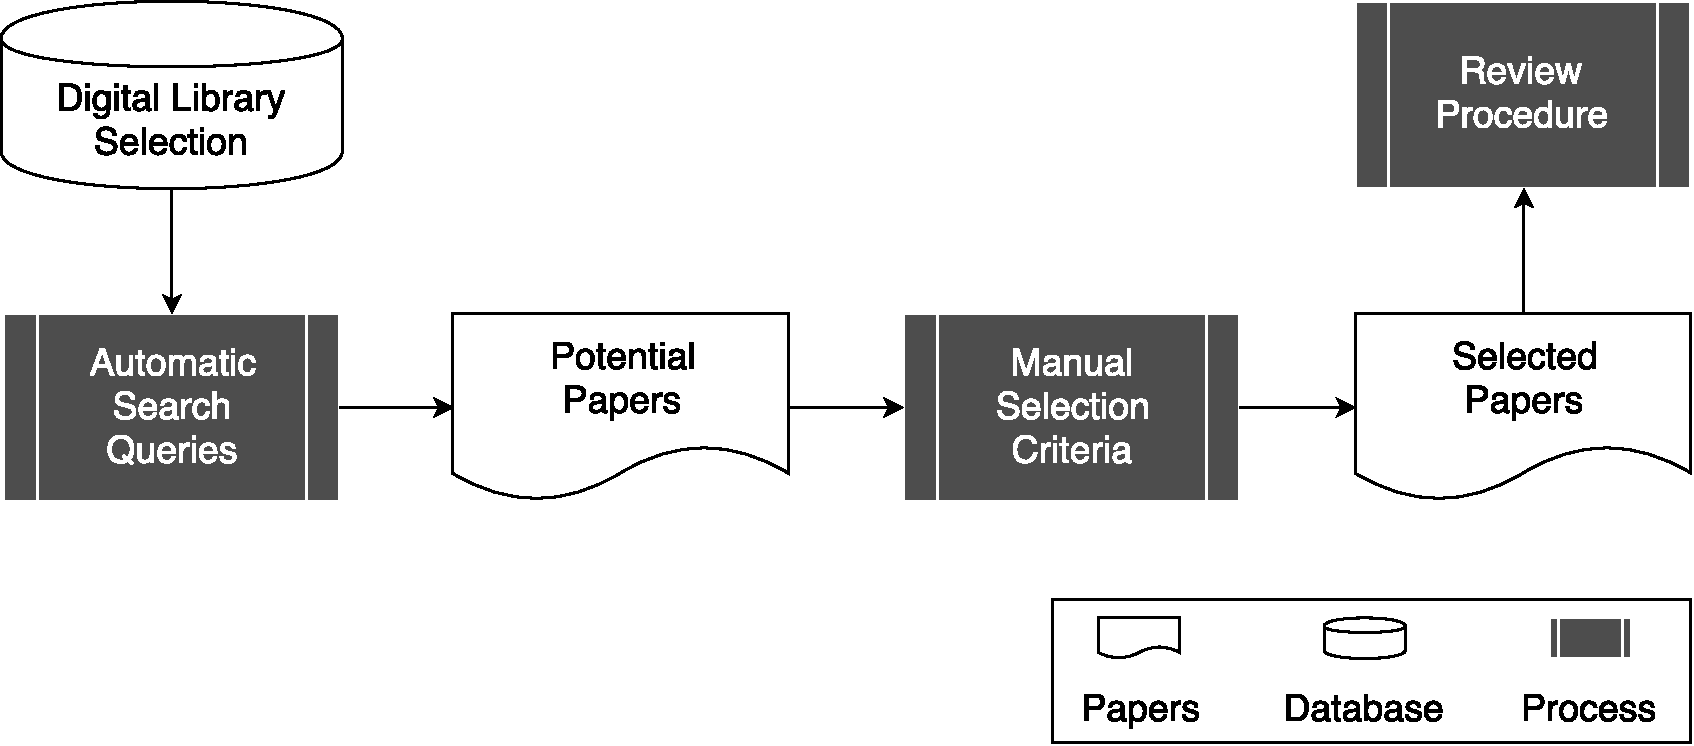
\includegraphics[width=6in]{litreview_process}
	\caption{\textbf{Literature Review Methods.}}
	\label{figure:litreview_process}
\end{figure}

\subsection{Event Detection} \label{event-detection}

x

\subsection{Event Prediction} \label{event-prediction}

x

\subsection{Visualization} \label{visualization}

x

\subsection{Applications} \label{applications}

x


% *** APPROACH ***


\section{Approach} \label{approach}

The


% *** RECENT PROGRESS ***


\section{Recent Progress} \label{recent-progress}

Recent progress involved the partial identification of several framework components and development of a small software package. The identified framework and software components are provided in Table \ref{table:frameworkcomponents} and \ref{table:softwarecomponents} respectively. A small software package was developed for Node.js \citep{Nodejs:2017} named \textit{"twitter2pg"}  \citep{Wen:2017} to conveniently extract real-time Twitter data into a relational PostgreSQL database \citep{Postgresql:2017}. The package has been downloaded 259 times as of December 2, 2017 after approximately a month of release, and consists of documentation, unit tests, and automatic Linux builds for continuous tests every month.

\begin{table}
\centering
\caption{\textbf{Identified Framework Objective Components.}}
\label{table:frameworkcomponents}
\begin{tabular}{|p{2in}|p{4in}|}
\hline
\textbf{Component} & \textbf{Identified} \\ \hline
Data Sources & Twitter Streaming API, Programmable Web \\ \hline
Data Structures & Unstructured (JSON), Location Points, Time Stamps \\ \hline
Event Detection Methods & Frequency, Sliding Window, Normalization, Clustering, Sampling, Graphs, Machine Learning \\ \hline
Output & Textual Summary, Webmap, Wordcloud \\ \hline
Use Cases & Influenza, Earthquake, Psychosocial, Energy, Traffic, Air Quality \\ \hline
\end{tabular}
\end{table}

\begin{table}
\centering
\caption{\textbf{Identified Software Objective Components.}}
\label{table:softwarecomponents}
\begin{tabular}{|p{2in}|p{4in}|}
\hline
\textbf{Component} & \textbf{Identified} \\ \hline
Databases & PostgreSQL, MongoDB, MySQL, Hbase, Cassandra, Accumulo, GeoMesa \\ \hline
Event Detection and Prediction Software & Massive Online Analysis (MOA), scikit-learn, Apache Spark/Kafka \\ \hline
Information Software & Leaflet, Carto, D3.js \\ \hline
Online Platform & Github, PyPi, npm \\ \hline
Testing Software & travis Continuous Integration (CI), Docker \\ \hline
Documentation Software & HTML, Markdown \\ \hline
\end{tabular}
\end{table}


% *** IMPACT ***


\section{Impact} \label{impact}

x


% *** CONCLUSION ***


\section{Conclusion} \label{conclusion}

x

